\documentclass[unicode,11pt,a4paper,oneside,numbers=endperiod,openany]{scrartcl}
\usepackage{amsmath} 
\usepackage{amsfonts}
\usepackage{graphicx}
\usepackage{enumitem} 
\usepackage{longtable}
\usepackage{array}
\usepackage{xcolor}
\usepackage{booktabs}
\usepackage{multirow}
\usepackage{geometry}
\usepackage{listings}
\lstdefinestyle{mystyle}{
    basicstyle=\ttfamily\small,
    keywordstyle=\color{blue},
    commentstyle=\color{green},
    stringstyle=\color{red},
    numbers=left,
    numberstyle=\tiny,
    stepnumber=1,
    frame=single,
    breaklines=true,
    captionpos=b,
    tabsize=2
}

\lstdefinelanguage{MyC++}{
    language=C++,
    morekeywords={std, vector, string},
}

\lstdefinelanguage{MyPython}{
    language=Python,
    morekeywords={self},
}

\lstdefinelanguage{MyBatch}{
    morekeywords={echo, pause, set},
    sensitive=false, 
    morecomment=[l]{REM}, 
    morestring=[b]",
}

\lstdefinelanguage{MyPython}{
    language=Python,
    morekeywords={self, int, float, str, list, dict, set, tuple, bool, None, True, False},
    keywordstyle=\color{blue},
    stringstyle=\color{red},
    commentstyle=\color{green},
    sensitive=true
}

\lstdefinelanguage{MyBash}{
    basicstyle=\ttfamily,
    breaklines=true,
    frame=single,
    keywordstyle=\color{blue},
    commentstyle=\color{gray},
    showstringspaces=false
}
\usepackage{ifthen}
\usepackage[utf8]{inputenc}
\usepackage{graphics}
\usepackage{graphicx}
\usepackage{hyperref}

\pagestyle{plain}
\voffset -5mm
\oddsidemargin  0mm
\evensidemargin -11mm
\marginparwidth 2cm
\marginparsep 0pt
\topmargin 0mm
\headheight 0pt
\headsep 0pt
\topskip 0pt        
\textheight 255mm
\textwidth 165mm

\newcommand{\duedate} {}
\newcommand{\setduedate}[1]{%
\renewcommand\duedate {See iCorsi for due date}}
\newcommand\isassignment {false}
\newcommand{\setassignment}{\renewcommand\isassignment {true}}
\newcommand{\ifassignment}[1]{\ifthenelse{\boolean{\isassignment}}{#1}{}}
\newcommand{\ifnotassignment}[1]{\ifthenelse{\boolean{\isassignment}}{}{#1}}

\newcommand{\assignmentpolicy}{
\begin{table}[h]
\begin{center}
\scalebox{0.8} {%
\begin{tabular}{|p{0.02cm}p{16cm}|}
\hline
&\\
\multicolumn{2}{|c|}{\Large\textbf{HPC Lab ---  Submission Instructions}}\\
\multicolumn{2}{|c|}{\large\textbf{(Please, notice that following instructions are mandatory: }}\\
\multicolumn{2}{|c|}{\large\textbf{submissions that don't comply with, won't be considered)}}\\
&\\
\textbullet & Assignments must be submitted to \href{https://www.icorsi.ch}{iCorsi} (i.e. in electronic format).\\
\textbullet & Provide both executable package and sources (e.g. C/C++ files, Matlab). 
If you are using libraries, please add them in the file. Sources must be organized in directories called:\\
\multicolumn{2}{|c|}{\textit{Project\_number\_lastname\_firstname}}\\
& and  the  file must be called:\\
\multicolumn{2}{|c|}{\textit{project\_number\_lastname\_firstname.zip}}\\
\multicolumn{2}{|c|}{\textit{project\_number\_lastname\_firstname.pdf}}\\
\textbullet &  The TAs will grade your project by reviewing your project write-up, and looking at the implementation 
                 you attempted, and benchmarking your code's performance.\\

\textbullet & You are allowed to discuss all questions with anyone you like; however: (i) your submission must list anyone you discussed problems with and (ii) you must write up your submission independently.\\
\hline
\end{tabular}
}
\end{center}
\end{table}
}
\newcommand{\punkte}[1]{\hspace{1ex}\emph{\mdseries\hfill(#1~\ifcase#1{Points}\or{Points}\else{Points}\fi)}}


\newcommand\serieheader[6]{
\thispagestyle{empty}%
\begin{flushleft}

\includegraphics[width=0.4\textwidth]{usi_inf.png}
\end{flushleft}
  \noindent%
  {\large\ignorespaces{\textbf{#1}}\hspace{\fill}\ignorespaces{ \textbf{#2}}}\\ \\%
  {\large\ignorespaces #3 \hspace{\fill}\ignorespaces #4}\\
  \noindent%
  \bigskip
  \hrule\par\bigskip\noindent%
  \bigskip {\ignorespaces {\Large{\textbf{#5}}}
  \hspace{\fill}\ignorespaces \large \ifthenelse{\boolean{\isassignment}}{\duedate}{#6}}
  \hrule\par\bigskip\noindent%  \linebreak
 }

\makeatletter
\def\enumerateMod{\ifnum \@enumdepth >3 \@toodeep\else
      \advance\@enumdepth \@ne
      \edef\@enumctr{enum\romannumeral\the\@enumdepth}\list
      {\csname label\@enumctr\endcsname}{\usecounter
        {\@enumctr}%%%? the following differs from "enumerate"
	\topsep0pt%
	\partopsep0pt%
	\itemsep0pt%
	\def\makelabel##1{\hss\llap{##1}}}\fi}
\let\endenumerateMod =\endlist
\makeatother




\usepackage{textcomp}





\begin{document}


\setassignment

\serieheader{High-Performance Computing Lab}{Institute of Computing}{Student: Zitian Wang}{Discussed with: None}{Solution for Project 5}{}
\newline

\assignmentpolicy
This project will introduce you a parallel space solution of a nonlinear PDE using MPI.

% -------------------------------------------------------------------------- %
% -------------------------------------------------------------------------- %
% ---------------------- Exercise 1 -----------------------------------------%
% -------------------------------------------------------------------------- %
% -------------------------------------------------------------------------- %

\section{Task 1 - Initialize and finalize MPI }

\begin{lstlisting}[style=mystyle, language=MyBash, caption={Execution of mini-stencil Simulation}]
    [wangzi@icsnode33 mini_app]$ mpirun ./main 128 100 0.005
    ========================================================
                          Welcome to mini-stencil!
    version   :: C++ MPI
    processes :: 4
    mesh      :: 128 * 128 dx = 0.00787402
    time      :: 100 time steps from 0 .. 0.005
    iteration :: CG 300, Newton 50, tolerance 1e-06
    =========================================================
    ---------------------------------------------------------
    1513 conjugate gradient iterations, at rate of 6599.61 iters/second
    300 newton iterations
    ---------------------------------------------------------
    Goodbye!
\end{lstlisting}

Limited condition \texttt{rank == 0 } to make sure only process 0 report in terminal.

\section{Task 2 - Create a Cartesian topology }

\begin{lstlisting}[style=mystyle, language=MyC++, caption={Setting Up a 2D Cartesian Topology with MPI}]
    // TODO: determine the number of sub-domains in the x and y dimensions
    //       using MPI_Dims_create
    int dims[2] = {1, 1};
    MPI_Dims_create(mpi_size, 2, dims);
    ndomy = dims[0];
    ndomx = dims[1];

    // TODO: create a 2D non-periodic Cartesian topology using MPI_Cart_create
    int periods[2] = {0, 0};
    MPI_Comm comm_cart;
    MPI_Cart_create(MPI_COMM_WORLD, 2, dims, periods, 0, &comm_cart);

    // TODO: retrieve coordinates of the rank in the topology using
    // MPI_Cart_coords
    int coords[2] = {0, 0};
    MPI_Cart_coords(comm_cart, mpi_rank, 2, coords);
    domy = coords[0] + 1;
    domx = coords[1] + 1;

    // TODO: set neighbours for all directions using MPI_Cart_shift
    MPI_Cart_shift(comm_cart, 0, 1, &neighbour_south, &neighbour_north);
    MPI_Cart_shift(comm_cart, 1, 1, &neighbour_west, &neighbour_east);
\end{lstlisting}

I used a \textbf{2D Cartesian domain decomposition} to divide the grid across MPI processes. \texttt{MPI\_Dims\_create} determined a balanced decomposition, and \texttt{MPI\_Cart\_create} established a non-periodic Cartesian topology for identifying neighboring subdomains.

Each process handles a specific subdomain, ensuring consistent workload distribution and efficient computation.

\subsection{Method selected reason}

\begin{enumerate}
    \item \textbf{Load Balancing}: Dividing the domain into equal-sized subdomains ensures each process has similar work, preventing load imbalance.
    \item \textbf{Communication Efficiency}: The 2D Cartesian topology allows efficient communication with only immediate neighbors, minimizing overhead.
    \item \textbf{Scalability}: This strategy scales well with increasing grid size or number of processes, maintaining balance and efficiency.
\end{enumerate}

\subsection{Implications on Performance}

\begin{enumerate}
    \item \textbf{Load Balancing}: \texttt{MPI\_Dims\_create} ensures even domain division, minimizing idle time and maximizing resource use.
    \item \textbf{Communication Overhead}: Communication is limited to neighboring processes, reducing data transfer and overall cost.
    \item \textbf{Computational Efficiency}: Each process independently handles a subdomain, allowing effective parallelization and overlapping of communication and computation.
\end{enumerate}


\section{Task 3 - Change linear algebra functions }

\begin{lstlisting}[style=mystyle, language=MyC++, caption={Implementation of \texttt{hpc\_dot} for Dot Product with MPI}]
    double hpc_dot(Field const& x, Field const& y) {
        double local_result = 0;
        int N = y.length();
    
        // Compute local result
        for (int i = 0; i < N; i++) {
            local_result += x[i] * y[i];
        }
    
        double global_result = 0;
        // Perform an MPI_Allreduce to sum up results across all processes
        MPI_Allreduce(&local_result, &global_result, 1, MPI_DOUBLE, MPI_SUM, MPI_COMM_WORLD);
    
        return global_result;
    }
\end{lstlisting}
    
\begin{lstlisting}[style=mystyle, language=MyC++, caption={Implementation of \texttt{hpc\_norm2} for 2-Norm Calculation with MPI}]
    double hpc_norm2(Field const& x) {
        double local_result = 0;
        int N = x.length();
    
        // Compute local result
        for (int i = 0; i < N; i++) {
            local_result += x[i] * x[i];
        }
    
        double global_result = 0;
        // Perform an MPI_Allreduce to sum up the squared values across all processes
        MPI_Allreduce(&local_result, &global_result, 1, MPI_DOUBLE, MPI_SUM, MPI_COMM_WORLD);
    
        // Return the square root of the global result
        return sqrt(global_result);
    }
\end{lstlisting}

\begin{lstlisting}[style=mystyle, language=MyC++, caption={Implementation of \texttt{hpc\_cg} for Conjugate Gradient Method}]
    void hpc_cg(Field& deltay, Field const& y_old, Field const& y_new,
                Field const& f, const int maxiters, const double tol,
                bool& success) {
        // This is the dimension of the linear system to solve
        int nx = data::domain.nx;
        int ny = data::domain.ny;
    
        if (!cg_initialized) cg_init(nx, ny);
    
        // Epsilon value for matrix-vector approximation
        double eps     = 1.e-4;
        double eps_inv = 1. / eps;
    
        // Initialize to zero
        hpc_fill(fv, 0.0);
    
        // Jacobian times deltay matrix-vector multiplication approximation
        // J*deltay = 1/epsilon * ( f(y_new + epsilon*deltay) - f(y_new) )
    
        // v = y_new + epsilon*deltay
        hpc_lcomb(v, 1.0, y_new, eps, deltay);
    
        // fv = f(v)
        diffusion(y_old, v, fv);
    
        // r = b - A*x = f(y_new) - J*deltay
        // where A*x = (f(v) - f) / eps
        hpc_add_scaled_diff(r, f, -eps_inv, fv, f);
    
        // p = r
        hpc_copy(p, r);
    
        // r_old_inner = <r, r>
        double r_old_inner = hpc_dot(r, r), r_new_inner = r_old_inner;
        MPI_Allreduce(MPI_IN_PLACE, &r_old_inner, 1, MPI_DOUBLE, MPI_SUM, MPI_COMM_WORLD);
    
        // Check for convergence
        success = false;
        if (sqrt(r_old_inner) < tol) {
            success = true;
            return;
        }
    
        int iter;
        for (iter = 0; iter < maxiters; iter++) {
            // Ap = A*p
            hpc_lcomb(v, 1.0, y_new, eps, p);
            diffusion(y_old, v, fv);
            hpc_scaled_diff(Ap, eps_inv, fv, f);
    
            // alpha = r_old_inner / p' * Ap
            double pAp = hpc_dot(p, Ap);
            MPI_Allreduce(MPI_IN_PLACE, &pAp, 1, MPI_DOUBLE, MPI_SUM, MPI_COMM_WORLD);
            double alpha = r_old_inner / pAp;
    
            // deltay += alpha * p
            hpc_axpy(deltay, alpha, p);
    
            // r -= alpha * Ap
            hpc_axpy(r, -alpha, Ap);
    
            // Find new norm
            r_new_inner = hpc_dot(r, r);
            MPI_Allreduce(MPI_IN_PLACE, &r_new_inner, 1, MPI_DOUBLE, MPI_SUM, MPI_COMM_WORLD);
    
            // Test for convergence
            if (sqrt(r_new_inner) < tol) {
                success = true;
                break;
            }
    
            // p = r + (r_new_inner / r_old_inner) * p
            double beta = r_new_inner / r_old_inner;
            hpc_lcomb(p, 1.0, r, beta, p);
    
            r_old_inner = r_new_inner;
        }
        stats::iters_cg += iter + 1;
    
        if (!success) std::cerr << "ERROR: CG failed to converge" << std::endl;
    }
\end{lstlisting}

\subsection{Functions Modified and Not Modified}

I modified several functions to enable parallel computation. The \textbf{hpc\_dot} function, responsible for inner product calculation, was updated to compute the local inner product within each process and then use \texttt{MPI\_Allreduce} to aggregate results globally. Similarly, the \textbf{hpc\_norm2} function for 2-norm calculation was modified to calculate the local sum of squares, aggregate using \texttt{MPI\_Allreduce}, and compute the square root of the global result. The \textbf{hpc\_cg} function is a Conjugate Gradient solver for solving large, sparse, symmetric positive-definite systems of linear equations from PDE discretization.For Jacobian matrix-vector multiplication, I implemented halo cell exchanges using non-blocking communication (\texttt{MPI\_Isend} and \texttt{MPI\_Irecv}) to ensure efficient handling of subdomain boundaries. Additionally, I updated the convergence check to use \texttt{MPI\_Allreduce} for global residual norm computation.

I did not modify the vector operations (\textbf{hpc\_axpy}, \textbf{hpc\_add\_scaled\_diff}, \textbf{hpc\_scaled\_diff}, \textbf{hpc\_scale}, \textbf{hpc\_lcomb} and \textbf{hpc\_copy}). These functions only involve local calculations within each process and do not require cross-process communication, so the original implementation was sufficient.

\subsection{Modification Method and Analysis}

For the inner product calculation (\textbf{hpc\_dot}), I ensured that each process computes the inner product of its local vector segment and then aggregates the results using \texttt{MPI\_Allreduce} to obtain the global value. This approach efficiently parallelizes the computation while ensuring consistency.

For the 2-norm calculation (\textbf{hpc\_norm2}), I applied a similar strategy. Each process calculates the sum of squares of its local vector elements, and \texttt{MPI\_Allreduce} aggregates these sums. The square root of the global result is then computed to finalize the norm calculation.

For the \textbf{hpc\_cg}, replaced standard dot product with an MPI-based version using \texttt{MPI\_Allreduce} for global aggregation. Added halo cell exchanges using non-blocking communication (\texttt{MPI\_Isend} and \texttt{MPI\_Irecv}) to handle subdomain boundaries efficiently. Convergence Check (hpc\_norm2), Used \texttt{MPI\_Allreduce} to compute the global residual norm after each iteration.

The modifications were designed to balance load and minimize communication overhead. Each process performs its share of the computation, ensuring that the workload is evenly distributed. Communication overhead is introduced by \texttt{MPI\_Allreduce} and halo cell exchanges, but these operations are essential for maintaining accuracy and consistency in parallel computations. Using non-blocking communication for boundary exchanges further optimizes performance by overlapping communication with computation.

\section{Task 4 - Exchange ghost cells [45 Points] }
\subsection{Ghost cell exchange function}
\begin{lstlisting}[style=mystyle, language=MyC++, caption={Non-Blocking Communication for Neighbor Exchange}]
    MPI_Request requests[8];
    int req_count = 0;
    
    // Send to and receive from the northern neighbor
    MPI_Isend(&s_new(0, jend-1), nx, MPI_DOUBLE, domain.neighbour_north, 0, MPI_COMM_WORLD, &requests[req_count++]);
    MPI_Irecv(&buffN[0], nx, MPI_DOUBLE, domain.neighbour_north, 1, MPI_COMM_WORLD, &requests[req_count++]);
    
    // Send to and receive from the southern neighbor
    MPI_Isend(&s_new(0, 0), nx, MPI_DOUBLE, domain.neighbour_south, 2, MPI_COMM_WORLD, &requests[req_count++]);
    MPI_Irecv(&buffS[0], nx, MPI_DOUBLE, domain.neighbour_south, 3, MPI_COMM_WORLD, &requests[req_count++]);
    
    // Send to and receive from the eastern neighbor
    MPI_Isend(&s_new(iend-1, 0), ny, MPI_DOUBLE, domain.neighbour_east, 4, MPI_COMM_WORLD, &requests[req_count++]);
    MPI_Irecv(&buffE[0], ny, MPI_DOUBLE, domain.neighbour_east, 5, MPI_COMM_WORLD, &requests[req_count++]);
    
    // Send to and receive from the western neighbor
    MPI_Isend(&s_new(0, 0), ny, MPI_DOUBLE, domain.neighbour_west, 6, MPI_COMM_WORLD, &requests[req_count++]);
    MPI_Irecv(&buffW[0], ny, MPI_DOUBLE, domain.neighbour_west, 7, MPI_COMM_WORLD, &requests[req_count++]);
    
    // Wait for all communication requests to complete
    MPI_Waitall(req_count, requests, MPI_STATUSES_IGNORE);
\end{lstlisting}

To exchange ghost cells between neighboring processes, I used \texttt{MPI\_Isend} and \texttt{MPI\_Irecv}, which allow overlapping communication with computation, improving efficiency. Each subdomain sends its boundary values to neighboring subdomains and receives boundary values from them. Communication is required for the north, south, east, and west boundaries. 

For each direction:
\begin{itemize}
    \item Initiate an \texttt{MPI\_Isend} to send the boundary values.
    \item Initiate an \texttt{MPI\_Irecv} to receive the ghost cell values.
\end{itemize}

After initiating all communications, I used \texttt{MPI\_Waitall} to ensure all communication had completed before proceeding with further calculations.
\subsection{Implement parallel I\//O}
\begin{lstlisting}[style=mystyle, language=MyBash, caption={Output of MPI Program for Distributed IO}]
    [wangzi@icsnode30 mpi_io]$ mpirun -np 4 ./mpi_io 100 100
    [Process  3 ( 1,  1)] global dims: 100 x 100; local dims: 50 x 50 (50:99 50:99);
    [Process  1 ( 0,  1)] global dims: 100 x 100; local dims: 50 x 50 (0:49, 50:99);
    [Process  0 ( 0,  0)] global dims: 100 x 100; local dims: 50 x 50 (0:49, 0:49);
    [Process  2 ( 1,  0)] global dims: 100 x 100; local dims: 50 x 50 (50:99, 0:49);
\end{lstlisting}
    
The demonstration code showcases the use of \textbf{MPI-IO} to write a distributed 2D grid into a single binary output file efficiently. The grid is decomposed across MPI processes, with each process handling a subdomain. The grid values are initialized to the MPI rank, and the data is written collectively to a binary file. Below are the main components:

\textbf{Domain Decomposition:} The global grid is divided into subdomains using a \texttt{2D Cartesian decomposition}. \texttt{MPI\_Dims\_create} determines the decomposition dimensions, while \texttt{MPI\_Cart\_create} creates a Cartesian topology to simplify communication and indexing. The \texttt{decomp1d} function ensures balanced workload distribution across processes.

\textbf{Memory Allocation and Initialization:} Each process allocates memory for its subdomain and initializes values to its MPI rank, enabling easy identification of ownership in the output.

\textbf{MPI-IO for Data Output:} 
\begin{itemize}
    \item \textbf{Subarray Types:} \texttt{MPI\_Type\_create\_subarray} defines the layout of each process’s subdomain within the global grid.
    \item \textbf{File View:} \texttt{MPI\_File\_set\_view} sets the global file view for each process, ensuring correct placement of data.
    \item \textbf{Collective Writing:} \texttt{MPI\_File\_write\_all} performs a collective I/O operation, ensuring synchronization and optimized performance.
\end{itemize}

\textbf{BOV File Creation:} After data writing, the root process generates a \textbf{BOV (Brick of Values)} header file, enabling visualization tools like \texttt{VisIt} to interpret the binary data correctly.

\textbf{Performance Considerations:} The domain decomposition ensures load balancing, while the use of MPI-IO and Cartesian topology supports scalability. Collective I/O minimizes file system contention, and derived datatypes ensure efficient data placement.

\subsection{Strong scaling}
\begin{figure}[h]
    \centering
    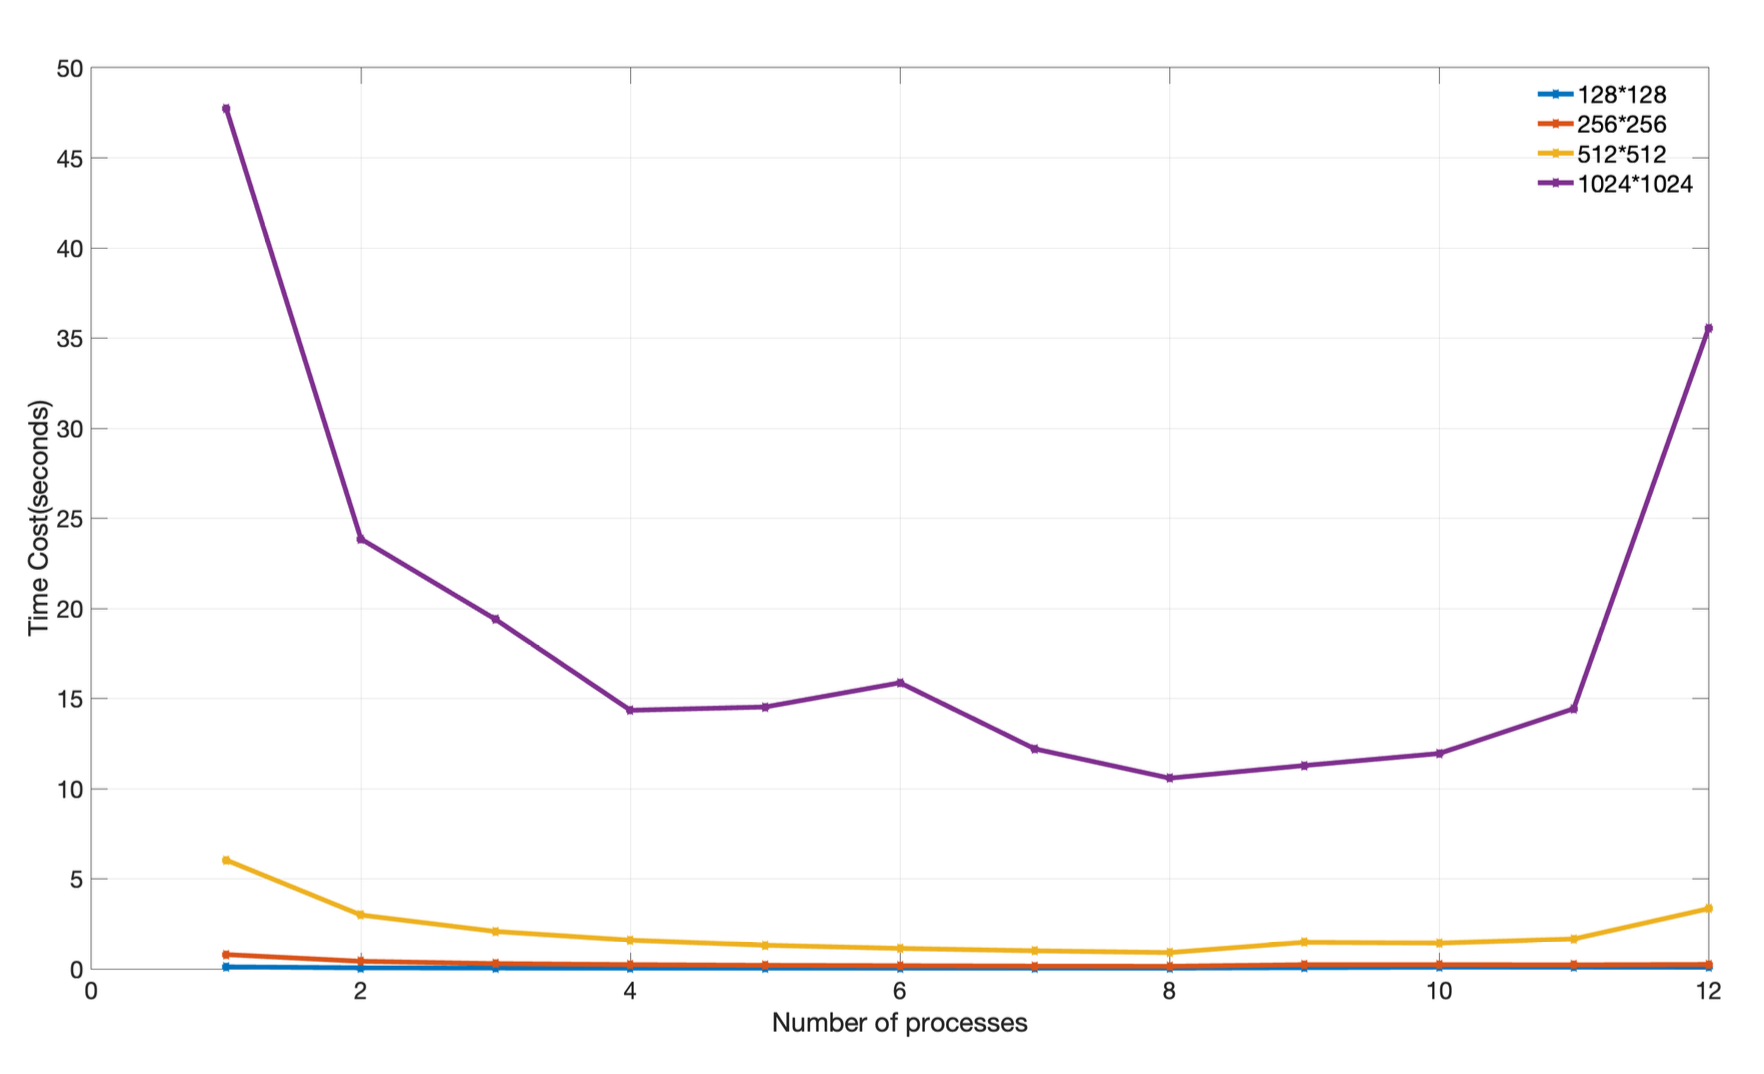
\includegraphics[width=0.5\textwidth]{pictures/strong.png}
    \caption{Strong scaling}
\end{figure}

Smaller resolutions (128 × 128, 256 × 256): When utilizing the parallel version of the PDE solver at these resolutions, performance does not improve and may even degrade. The reason for this condition might be that numerical procedures at this resolutions are computationally inexpensive. The parallel approach may even reduce performance owing to the expense of generating and managing threads.

Higher resolutions (e.g., 512 × 512 and 1024 × 1024) improve speed by employing several threads. The improvement is most noticeable at 1024 × 1024 resolution. Larger grid sizes are computationally more costly than smaller grids. In certain cases, the parallel version can greatly improve performance. The non-linear time cost can be ascribed to the trade-off between the expense of managing processes and the benefits derived from employing numerous processes.


\subsection{Weak scaling}
\begin{figure}[h]
    \centering
    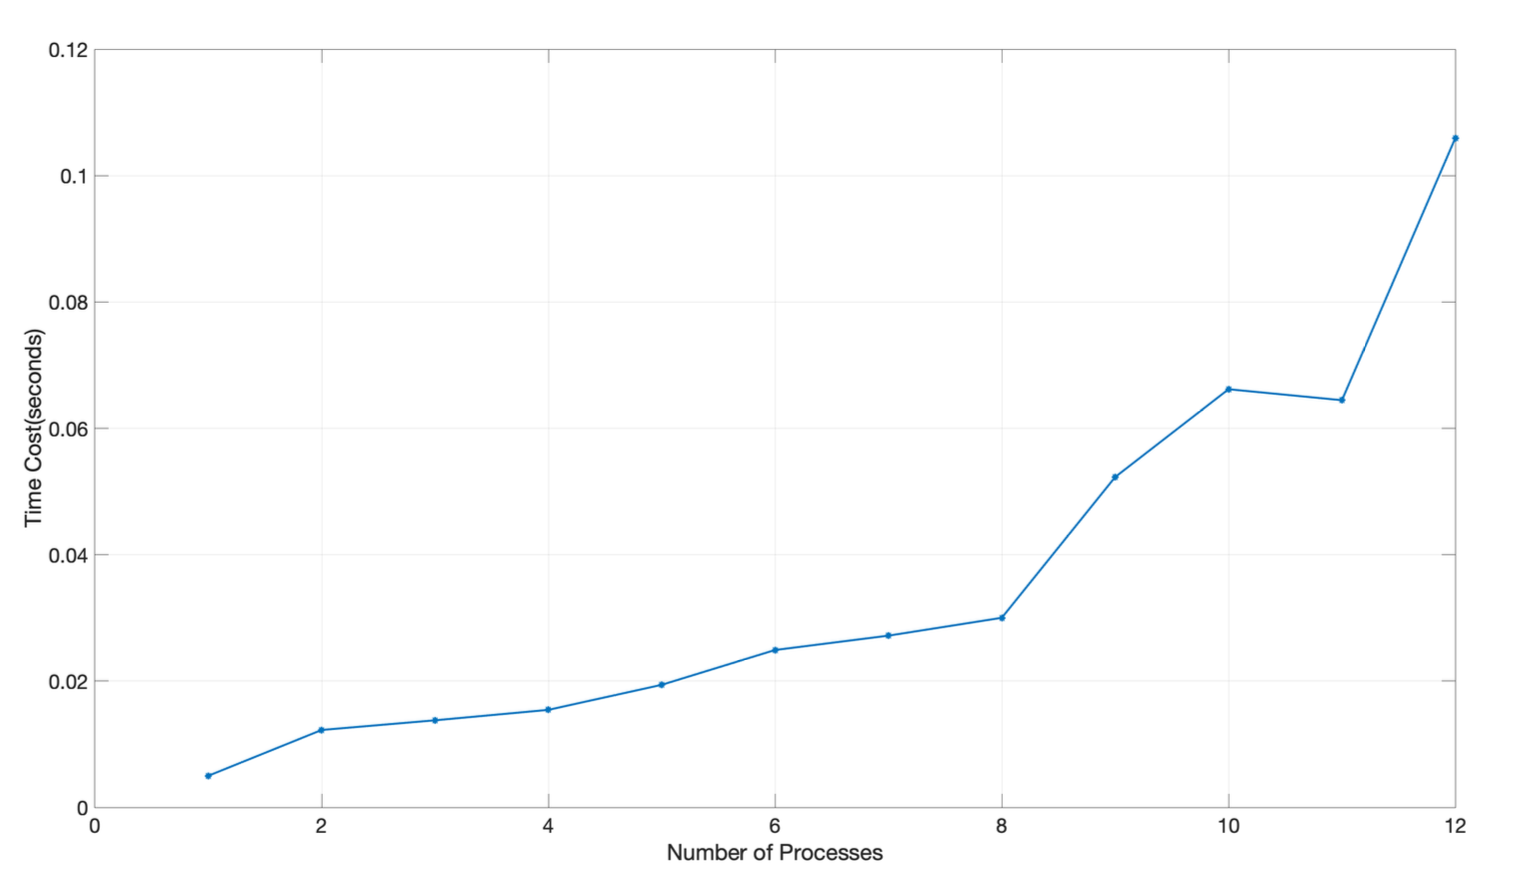
\includegraphics[width=0.5\textwidth]{pictures/weak.png}
    \caption{Weak scaling}
\end{figure}

The result is that as the number of processes increases, the time cost will rise proportionally. The reason for this is that, while increasing the number of processes, the communication overhead associated with the greater problem size is computationally expensive, resulting in an increase in time consumed. Furthermore, increasing the number of nonlinear iterations can degrade the PDE solver's performance.

\section{Task 5 - Testing}
\subsection{Sum of ranks: MPI collectives}
\begin{lstlisting}[language=MyPython, style=mystyle, caption={MPI-based Sum of Ranks Calculation in Python}]
    sum_of_ranks = comm.allreduce(rank, op=MPI.SUM)
    if rank == 0:
        print(f"Sum of all ranks (pickle-based): {sum_of_ranks}")
    comm.Barrier()
    
    rank_array = np.array(rank, dtype='i')
    sum_array = np.zeros(1, dtype='i')
    comm.Allreduce([rank_array, MPI.INT], [sum_array, MPI.INT], op=MPI.SUM)
\end{lstlisting}

\subsection{Ghost cell exchange between neighboring processes }
\begin{lstlisting}[language=MyPython, style=mystyle, caption={Creating a 2D Cartesian Topology in MPI}]
    dims = MPI.Compute_dims(size, [0, 0])
    rows, cols = dims
    periodic = [True, True]  
    reorder = False          
    cart_comm = comm.Create_cart(dims, periods=periodic, reorder=reorder)
    coords = cart_comm.Get_coords(rank)
    north, south = cart_comm.Shift(0, 1)
    east, west = cart_comm.Shift(1, 1)
\end{lstlisting}
\subsection{ A self-scheduling example: Parallel Mandelbrot}
\begin{lstlisting}[language=MyPython, style=mystyle, caption={Manager-Worker Model in MPI}]
    def manager(comm, tasks):
        completed = []
        num_workers = comm.Get_size() - 1
        for worker_id in range(1, num_workers + 1):
            comm.send(tasks[worker_id - 1], dest=worker_id, tag=TAG_TASK)
        for task_index in range(num_workers, len(tasks)):
            finished = comm.recv(source=MPI.ANY_SOURCE, tag=MPI.ANY_TAG)
            completed.append(finished)
            comm.send(tasks[task_index], dest=finished.Get_source(), tag=TAG_TASK)
        for _ in range(1, num_workers + 1):
            final_task = comm.recv(source=MPI.ANY_SOURCE, tag=MPI.ANY_TAG)
            completed.append(final_task)
            comm.send(None, dest=final_task.Get_source(), tag=TAG_DONE)
        return completed
    
    def worker(comm):
        task_flag = -1
        tasks_processed = 0
        while task_flag != TAG_DONE:
            task = comm.recv(source=MANAGER, tag=MPI.ANY_TAG)
            task_flag = task.Get_tag()
            if task_flag != TAG_DONE:
                task.process()
                comm.send(task, dest=MANAGER, tag=TAG_TASK_DONE)
            tasks_processed += 1
        return tasks_processed
 \end{lstlisting}
    
\end{document}
